\documentclass[11pt]{amsart}


\usepackage[ibidtracker=false,uniquename=false,giveninits=true,terseinits=true,backend=biber]{biblatex}
\usepackage{float}
\usepackage{graphicx}
\usepackage{todonotes}
\usepackage{subcaption}
\usepackage{amsmath}
\usepackage{amsthm}
\usepackage{amssymb}
\usepackage{algorithm}
\usepackage[noend]{algorithmic}
\usepackage[foot]{amsaddr}
\usepackage[misc]{ifsym}
\usepackage{enumitem}
\usepackage{geometry}
\usepackage[hidelinks]{hyperref}

\renewbibmacro{in:}{}
\addbibresource{rnni_geometry.bib}
\AtEveryBibitem{
	\clearlist{language}
}

\setlist{leftmargin = 0pt}
\geometry{margin=1in}


\newtheorem{proposition}{Proposition}
\newtheorem{theorem}{Theorem}
\newtheorem{lemma}{Lemma}
\newtheorem{corollary}{Corollary}
\newtheorem{problem}{Problem}
\newtheorem{conjecture}{Conjecture}

\newcommand{\lemmaautorefname}{Lemma}
\newcommand{\corollaryautorefname}{Corollary}
\renewcommand{\sectionautorefname}{Section}

\newcommand{\tocite}{ {\color{red}\fbox{CITATION}} }
\newcommand{\toref}{ {\color{blue}\fbox{Reference}} }
\newcommand{\rnni}{\mathrm{RNNI}}
\newcommand{\findpath}{\textsc{FindPath}}
\newcommand{\mrca}{\mathrm{mrca}}
\newcommand{\rank}{\mathrm{rank}}
\newcommand{\ntime}{\mathrm{time}}
\newcommand{\nni}{\mathrm{NNI}}
\newcommand{\spr}{\mathrm{SPR}}
\newcommand{\tbr}{\mathrm{TBR}}
\newcommand{\fp}{\mathrm{FP}}
\newcommand{\dtt}{\mathrm{DtT}}
\newcommand{\np}{\mathbf{NP}}
\newcommand{\decprob}[1]{\rnni(#1)\text{-}\mathrm{SP}}
\newcommand{\rad}{\mathit{rad}}
\renewcommand{\O}{\mathcal O}
\renewcommand{\epsilon}{\varepsilon}
\renewcommand{\thesubfigure}{\Alph{subfigure}}

\newcommand{\algorithmautorefname}{Algorithm}

\newcommand{\summary}[1]{\textbf{#1}} % Print summaries to .pdf
% \newcommand{\summary}[1]{} % Hide summaries in .pdf

\newcommand{\todefine}[1]{{\color{blue}{We need to define:#1}}} % Print summaries to .pdf

\DeclareMathOperator*{\argmin}{argmin}
\DeclareMathOperator*{\argmax}{argmax}

\graphicspath{{figures/}}

\sloppy


\title[Geometry of ranked tree spaces]{The Geometry of the Ranked Nearest Neighbour Interchange Space}
\date{\today}
\author{Lena Collienne}
\email{lcollienne@cs.otago.ac.nz}
\address{Department of Computer Science, University of Otago, New Zealand}
\author{Alex Gavryushkin\textsuperscript{\Letter}}
\email{\textsuperscript{\Letter}alex@biods.org}
\thanks{}

\begin{document}

\begin{abstract}
\end{abstract}

\maketitle


\section{Introduction}

\todo{Include Alex's idea from github issue \#1}
\summary{Why we want time-trees}

\summary{Why discrete time-trees -- Summarising for example}

\summary{How recent results about $\rnni$ make this space interesting and that it is strongly connected to $\dtt_m$}

\summary{Why we want to investigate geometrical properties of $\dtt_m$ and $\rnni$, and also $\rnni(\rho)$}

\summary{Structure of the paper.}


\section{Technical Introduction}

\summary{Introducing discrete time-trees and ranked trees}
A binary rooted phylogenetic tree is a binary tree on a fixed number $n$ of leaves, which are uniquely labelled by elements of the set $\{a_1, \ldots, a_n\}$.
The main objective of study in this paper, \emph{discrete time-trees}, are such binary rooted phylogenetic trees, where nodes are assigned \emph{times}, which are positive integers.
More specifically, all leaves are assigned time $0$, and every internal nodes is assigned a unique time, such that it always has time greater than its children.
We denote the time of an internal node $v$ by $\ntime(v)$.
If not stated otherwise, we refer to discrete time-trees simply as \emph{trees}.
We furthermore call two trees 
\todo{We need 'identical' for non-binary trees in the definition of the $\nni$ move. Is this confusing here or can we keep it like this?}
(not necessarily binary) \emph{identical} if there is a graph isomorphism between them preserving leaf labels and times.
The number of discrete time-trees with root time less or equal to $m$ is $\frac{(n-1)!n!m^{n-1}}{2^{n-1}}$ \autocite{Gavryushkin2018-ol}.

As special case of discrete time-trees are \emph{ranked trees} where the root has time $n-1$.
Then internal nodes are uniquely labelled by times in $\{1, \ldots, n-1\}$, and hence this definition of ranked trees coincides with the one of \textcite{Collienne2020-iu}.
In the case of ranked trees we say \emph{rank} of a node $v$ to mean its time ($\rank(v) = \ntime(v)$) to be consistent with notations used in \autocite{Collienne2020-iu}.

Every internal node $v$ of a tree $T$ can be referred to by the set $C$ of leaves that are descending from this node.
We call such a set $C$ \emph{cluster} and say that the cluster $C$ is \emph{induced} by $v$.
A list of clusters $[C_1, \ldots, C_{n-1}]$ uniquely defines a ranked tree, where cluster $C_i$ is induced by the internal node with rank $i$ for $i \in \{1, \ldots, n-1\}$.
For each subset $S \subseteq \{a_1, \ldots, a_n\}$ we call the internal node of a tree $T$ with lowest time that is ancestral to all elements of $S$ the \emph{most recent common ancestor} of $S$ and denote it by $(S)_T$.
\todo{Do we need the definition of $(T)_i$? It currently only appears in the FP pseudo-code}
We denote the parent of a leaf $a_i$ in $T$ by $(a_i)_T$, and the cluster induced by the node with time $i$ in $T$ by $(T)_i$.

\summary{Defining the tree space $\dtt_m$ and $\rnni = \dtt_{n-1}$}
We are now ready to introduce the centre of study in this paper, the graph (or space) of discrete time-trees.
This graph is called $\dtt_m$ for a fixed positive integer $m$.
The vertex set of $\dtt_m$ is the set of trees with root time less or equal to $m$.
Trees $T$ and $R$ are connected by an edge in this graph if performing one of the following (reversible) operations on $T$ results in $R$:
\begin{enumerate}
	\item An \emph{$\nni$ move} connects trees $T$ and $R$ if there is an edge $e$ in $T$ and an edge $f$ in $R$, both of length one, such that shrinking $e$ and $f$ to nodes results in identical trees.
	\item A \emph{rank move} on $T$ exchanges the times of two internal nodes with time difference one.
	\item A \emph{length move} on $T$ changes the time of an internal node by one.
\end{enumerate}
A length move can only change the time of a node to become $t$ if there is no node with time $t$ already.
Note that our definition of $\dtt_m$ differs from the definition of \textcite{Gavryushkin2018-ol}, as length move are defined differently in their paper.

We will say that a tree $T$ is neighbour of $R$ if the two trees are connected by an edge in $\dtt_m$.
The definition of $\dtt_m$ leads to a natural definition of the \emph{distance} between two trees $T$ and $R$ in this graph as the length of a shortest paths between these trees, denoted by $d(T,R)$.
We also consider the ranked nearest neighbour interchange ($\rnni$) graph of \textcite{Collienne2020-iu}, which is the graph $\dtt_m$ for $m=n-1$, and hence a graph of ranked trees.
In this graph length moves are not possible, so we use the notion $\rnni$ \emph{move} to mean either a rank move or an $\nni$ move to distinguish these moves from length moves.

\todefine{
	\begin{itemize}
		\item we refer to leaves by their label (necessary?)
		\item ($\rnni$) neighbour
		\item We need to mention that $m$ is fixed when we compute distances between two trees
		\item $\rnni(\rho)$ -- in corresponding section
		\item intervals -- only needed in $\rnni(\rho)$ section (e.g. for Lemma~\ref{lemma:nni_path_to_caterpillar})
		\item $(T)_i$ for cluster induced by node of rank $i$ in $T$ -- this is only needed for proofs around $\rnni(\rho)$ and in the proof that every tree is connected to a caterpillar tree in $\rnni$ by a sequence of $\nni$ moves AND $\findpath$ pseudo-code (!)
		\item We sometimes say $\rnni$ instead of $\rnni$ space. If we keep that, we might want to mention that we do it? -- We use just '$\rnni$' in polynomial paper as well!
		\item distinguish the shortest path problem from the distance problem! -- maybe mention that $\findpath$ is optimal algorithm for shortest path problem
	\end{itemize}
}


\section{Computing Shortest Paths in $\dtt_m$}
\label{section:fp_dtt}

\summary{Introduce how we can use $\findpath$ to compute $\dtt_m$ distances}
Distances between trees in $\rnni$ can be computed in quadratic running time with the algorithm $\findpath$, introduced by \textcite{Collienne2020-iu}.
As $\rnni$ is a special case of $\dtt_m$ for $m = n-1$, the question whether this algorithm can also be used to compute distances in $\dtt_m$ arises.
In this section we present a generalisation of $\findpath$ that computes distances between trees in $\dtt_m$.
Before introducing the version of $\findpath$ for $\dtt_m$, we introduce a way to convert trees in $\dtt_m$ into ranked trees, such that the $\rnni$ distance between those ranked trees equals their distance in $\dtt_m$ (\autoref{thm:dtt_findpath}).

\summary{How to add leaves to a $\dtt_m$ tree to transform it into a ranked tree}
Therefore, we consider trees $T$ and $R$ and construct ranked trees $T_r$ and $R_r$ as follows.
Let $m$ be the maximum root time of $T$ and $R$.
To receive a ranked tree $T_r$ on $m+2$ leaves from $T$, we add leaves to $T$ as described in the following (\autoref{alg:ranked_tree}).
The same is done for $R$ to get a ranked tree $R_r$.
To construct $T_r$, consider the tree $T$ and add a new root with time $m + 1$ that becomes parent of the root of $T$.
\todo{Define caterpillar tree (in technical intro?!)}
The second child of this new root is the root of a caterpillar tree on leaf set $\{a_{n+1}, a_{n+2}, \ldots, a_{m+2}\}$, such that $\ntime(a_{n+1}) = \ntime(a_{n+2}) < \ntime(a_{n+3}) < \ldots < \ntime(a_{m+2})$.
Hence $T_r$ is a uniquely defined ranked tree with $m+2$ leaves.
An example of this extension of a tree $T$ to a ranked tree $T_r$ is depicted in \autoref{fig:dtt_to_ranked_tree}.
Throughout this paper we use the index $r$ for $T_r$ to refer to this extended ranked version of any tree $T$.
Moreover, we denote the subtree of $T_r$ that is identical to $T$ by $T_r^d$ ($d$ for discrete time-tree) and the added caterpillar tree by $T_r^c$.

\begin{algorithm}[ht]
	\caption{RankedTree($T$)}
	\label{alg:ranked_tree}
	\begin{algorithmic}[1]
		\STATE $S:= \{1 \leq i \leq m | \text{ no internal node in } T \text{ has time } i\}$
		\STATE $[i_1, \ldots, i_{m-n+1}] = sort(S)$
		\STATE $T_r := T$ with additional internal node $v_1$ with children $a_{n+1}, a_{n+2}$ and time $i_1$
		\FOR {$k = 2, \dots, m-n+1$}
			\STATE Add internal node $v_k$ with with children $v_{k-1}$ and $a_{n+k+1}$ and time $i_k$ to $T_r$
		\STATE add internal node $\rho$ with children $v_{m-n}$ and $(\{a_1, \ldots, a_n\})_{T_r}$ to $T_r$
		\ENDFOR
		\RETURN $T_r$
	\end{algorithmic}
\end{algorithm}

\begin{figure}[ht]
	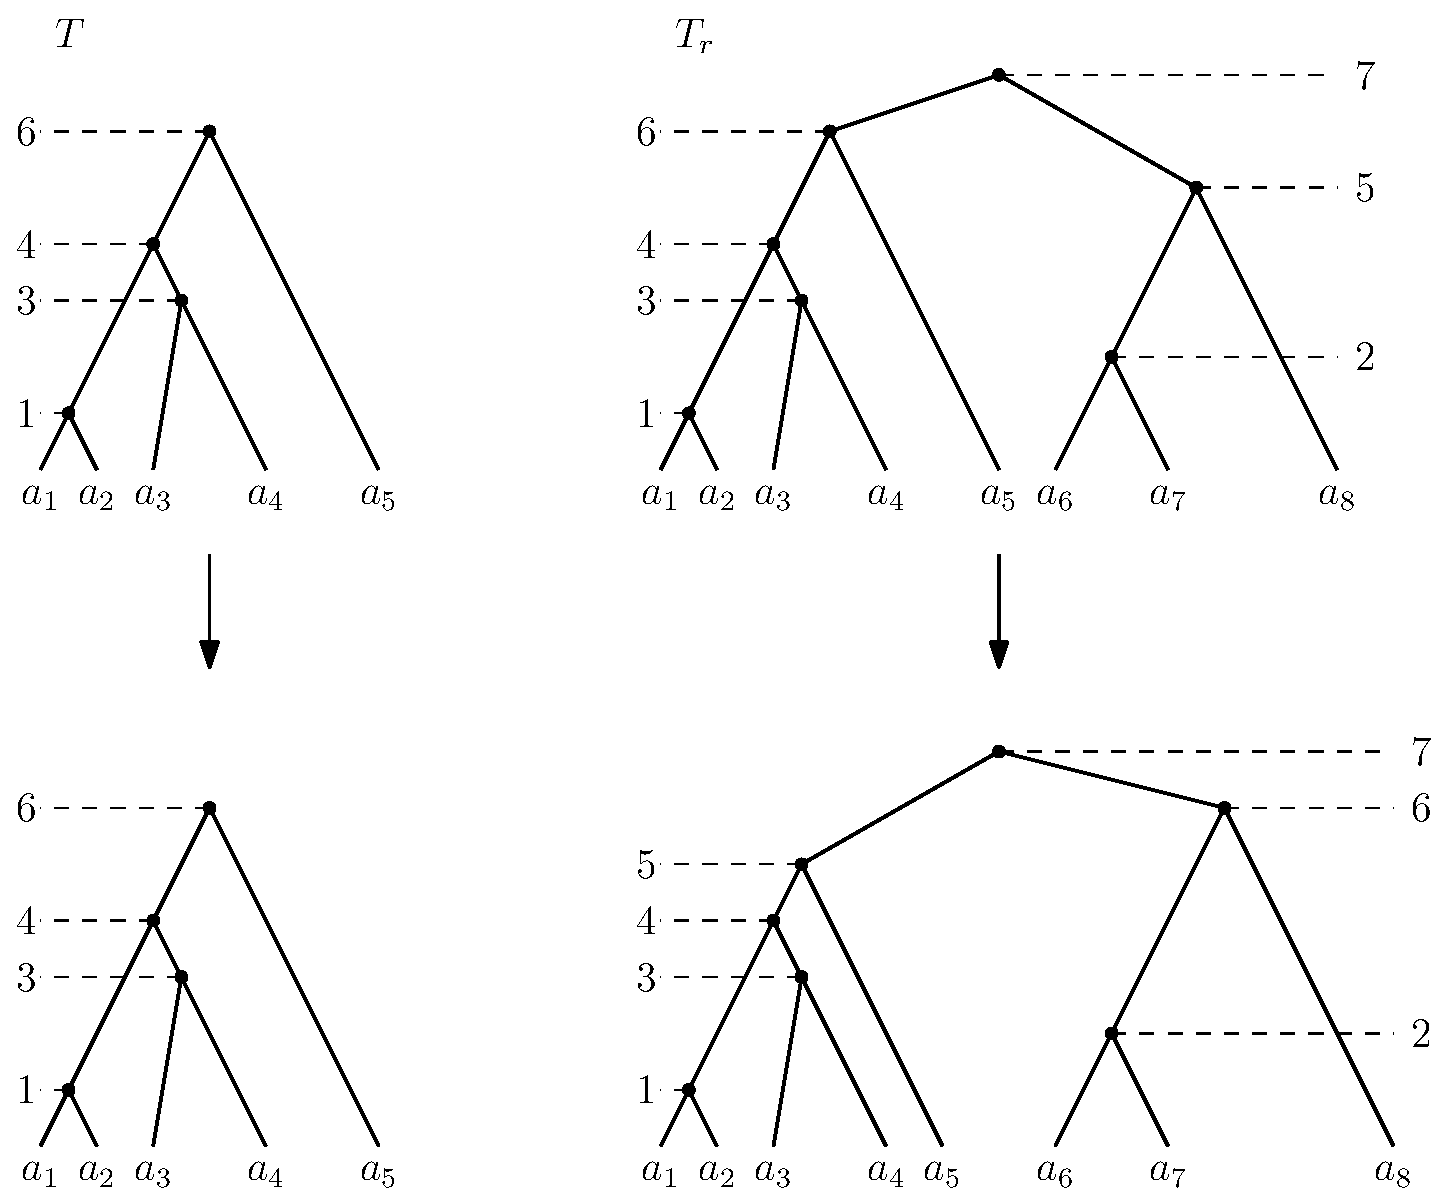
\includegraphics[width=0.75\textwidth]{dtt_to_ranked_tree.eps}
	\caption{Extending a tree $T$ on $n$ leaves in $\dtt_6$ (left) to a ranked tree with $m+2=8$ leaves (right) by adding a caterpillar subtree with three leaves.}
	\label{fig:dtt_to_ranked_tree}
\end{figure}

\summary{Moves on the extended ranked versions of trees -- $\rnni$ vs length moves}
In the following we distinguish not only rank moves and $\nni$ moves on the extended ranked version $T_r$ of a tree $T$, but we will also distinguish different types of rank moves.
Rank moves between one node of $T_c$ and one node of $T_d$ can be interpreted as length moves, as such rank moves can be seen as length moves in the subtree $T_d$ (\autoref{fig:rank_move_length_move.eps}).
All remaining rank moves will still be called rank moves.

\summary{How to compute shortest $\dtt_m$-paths between trees with $\findpath$}
After extending both trees $T$ and $R$ to ranked trees $T_r$ and $R_r$ on $m+2$ leaves, respectively, we can compute shortest paths between $T_r$ and $R_r$ in $\rnni$, using $\findpath$.
A path computed by $\findpath$ preserves clusters \autocite{Collienne2020-iu}, hence there are no $\nni$ moves in the newly added caterpillar tree with leaves in $\{a_{n+1}, \ldots, a_{m+2}\}$ on such a path.
The only moves involving internal nodes of this caterpillar subtree are rank moves that correspond to length moves, as described above.
Hence the path $\fp(T_r,R_r)$ provides a path between $T$ and $R$ in $\dtt_m$, when only considering the subtrees induced by $\{a_1, \ldots, a_n\}$ in all trees on $\fp(T_r, R_r)$, and interpreting some rank moves between $T_r$ and $R_r$ as length moves.
We denote this path in $\dtt_m$, which results from $\fp(T_r, R_r)$, by $\fp(T,R)$.
In \autoref{thm:dtt_findpath} we establish that $\fp(T,R)$ is a shortest path in $\dtt_m$ indeed.
Note that for any given pair of trees $T$ and $R$ we always assume $m$ to be the maximum root time of these trees in and aim to compute a shortest path between them in $\dtt_m$. 

\begin{theorem}
	The path $\fp(T,R)$ between two discrete time-trees $T$ and $R$ is a shortest path in $\dtt_m$, where $m$ is the maximum root time of $T$ and $R$.
	\label{thm:dtt_findpath}
\end{theorem}

\begin{proof}
	Let $T$ and $R$ be discrete time-trees and $T_r$ and $R_r$ their extended ranked versions computed with \autoref{alg:ranked_tree}, respectively.
	We have already seen above that, if interpreting some rank moves on the extended ranked versions of trees as length moves, a path computed by $\findpath$ can be seen as a path between discrete time-trees.
	It is also possible to convert a path between discrete time-trees to a path between their extended ranked versions by replacing length moves with rank moves, analogous to how it is described above, while all other moves stay the same.
	Therefore, any path in $\dtt_m$ from $T$ to $R$ gives a path of equal length between $T_r$ and $R_r$ in the $\rnni$ space on $m+2$ leaves.
	If there was a path between $T$ and $R$ shorter than $\fp(T,R)$, the corresponding path between $T_r$ and $R_r$ in $\rnni$ would be shorter than the one computed by $\findpath$ in this space.
	Since this contradicts \autocite[Theorem 1]{Collienne2020-iu}, it follows that $\fp(T,R)$ is a shortest path in $\dtt_m$.
\end{proof}

\summary{Running time of $\findpath$ + we don't need to add subtree in practice}
\autoref{thm:dtt_findpath} shows that $\findpath$ (\autoref{alg:fp_dtt}) computes shortest path between two trees in $\dtt_m$ in polynomial time, more specifically in $\O(mn)$, more details on this are provided following \autoref{thm:dtt_diameter}.
It is not even necessary to convert a given pair of discrete time-trees to ranked trees to apply $\findpath$ on them.
Instead, we can define a modified version of $\findpath$ for trees in $\dtt_m$.
Therefore, iterations of $\findpath$ on the ranked trees that consider clusters in the added caterpillar trees are replaced by length moves increasing the time of internal nodes as described in the \textbf{for} loop in Line~\ref{line:length_move} of \autoref{alg:fp_dtt}.
The benefit of this modified version of the algorithm, compared to using $\findpath$ on the extended ranked versions of the trees, is a reduced use of memory, which is especially of practical relevance for $m >> n$.

Throughout this paper we will however consider $\findpath$ applied to the extended ranked versions of discrete time-trees, as this simplifies some proofs.

\begin{algorithm}[h]
	\caption{$\findpath$($T,R$)}
	\begin{algorithmic}[1]
		\label{alg:fp_dtt}
		\STATE $T_1 := T$, $p := [T_1]$
		\FOR {$k = 1, \dots, m$}
			\IF {$R$ has a node with rank $i$}
			\STATE $C:=(R)_i$
			\WHILE {$\rank((C)_{T_1})>k$}
					\STATE $T_2$ is $T_1$ with the rank of $(C)_{T_1}$ decreased by an $\rnni$ move
				\STATE $T_1 = T_2$
				\STATE $p = p+T_1$
			\ENDWHILE
			\ELSE
				\STATE $i := \min\{l | l>k \text{ and no node in } T_1 \text{ has time }l\}$
				\FOR {$j = i-1, \dots, k$}
					\label{line:length_move}
					\STATE $T_2$ is $T_1$ where the time of $(T_1)_j$ is increased by one (length move)
					\STATE $T_1 = T_2$
					\STATE $p = p+T_1$
				\ENDFOR
			\ENDIF
		\ENDFOR
		\RETURN $p$
	\end{algorithmic}
\end{algorithm}


\section{Geometrical Properties of $\dtt_m$}

\subsection{Cluster Property}
\summary{Definition of Cluster Property and why it is relevant (a bit of bio).}
In this section we consider a property of tree spaces that is of relevance because of its biological meaning and its connection to complexity results in a tree space similar to $\rnni$.
We say that a tree space has the \emph{cluster property}, if all trees on every shortest paths between two trees sharing a cluster $C$ also contain this cluster.
This is desirable biological property as for example for a given sample of trees containing a common subtree, it is expected a summary or mean tree of the sample also contains this subtree.

\summary{Cluster property in $\nni$ and its connection to the complexity result.}
A tree space very similar to $\rnni$, that has been studied extensively \tocite is the $\nni$ graph on trees without times where $\nni$ moves are allowed on every edge.
Computing distances in $\nni$ is $\np$-hard\autocite{Dasgupta2000-xa}, and the proof relies on the fact that this tree space does not have the cluster property \autocite{Li1996-zw}.
In the $\rnni$ graph, however, distances can be computed in polynomial time by the algorithm $\findpath$ \autocite{Collienne2020-iu}, which preserves common clusters.
The question whether $\rnni$ has the cluster property is hence natural, and will be settled in \autoref{thm:cluster_property_rnni}.
\todo{Does $\spr$ have the cluster property?}
Note that even though it seems like distances can be computed in polynomial time in a tree space if it has the cluster property, this does not need to be true in general.

\summary{$\rnni$ has the cluster property.}
\begin{theorem}
	The $\rnni$ graph has the cluster property.
	\label{thm:cluster_property_rnni}
\end{theorem}

\begin{proof}
	We assume to the contrary that there are two ranked trees sharing a cluster that are connected by a shortest path that does not preserve this cluster.
	Let $T$ and $R$ be ranked trees with minimal distance among those, with shared cluster $C$ that is not present in every tree on a shortest path $p$ between $T$ and $R$.
	Because of this minimality assumption on the length of $p$, the first tree $T'$ after $T$ on $p$ does not contain $C$.
	Therefore, all nodes with rank below $(C)_T$ induce the same clusters in $T$ and $T'$.
	We now compare the distances $d(T,R)$ and $d(T',R)$ by comparing paths $\findpath$ computes between $T$ and $R$ with those computed between $T'$ and $R$.

	All trees on $\fp(R,T)$ and $\fp(R, T')$ coincide until the point is reached where the cluster that is considered by $\findpath$ on $R$ and $T$ is $C$.
	Let $\hat T$ denote the tree right before cluster $C$ is considered.
	Then $\fp(R,T)$ and $\fp(R,T')$ coincide up to this tree $\hat T$.
	It follows $d(T,R) = d(R,\hat T) + d(\hat T, T)$ and $d(T',R) = d(R,\hat T) + d(\hat T, T')$.

	Now consider $\fp(T', \hat T)$, which has length $d(\hat T, T')$.
	As $\findpath$ preserves clusters, $C$ is present in every tree on $\fp(T,R)$ up to and including $\hat T$.
	The fist iteration of $\findpath$ applied to the pair of trees $(T',\hat T)$ considers the cluster $C$, as all cluster induced by nodes below $(C)_{T'}$ coincide in $\hat T$ and $T'$.
	\todo{Do we need a figure here?}
	To construct the cluster $C$ in $T'$, there is just one $\nni$ move needed, which results in the tree $T$, as $T$ and $T'$ are $\nni$ neighbours such that $T$ contains $C$ and $T'$ does not.
	We can therefore conclude that $d(T,R) = d(T',R) - 1$, which contradicts the assumption that $T'$ is the first tree on a shortest path from $T$ to $R$.
	Hence, there is no shortest path between $T$ and $R$ that does not preserve $C$ which shows that the $\rnni$ graph has the cluster property.
\end{proof}

The fact that a slightly modified version of $\findpath$ computes shortest paths $\dtt_m$ already suggest that there is a close relation between shortest path in $\rnni$ and $\dtt_m$.
With the following lemma we see that any shortest path in $\dtt_m$ provides a shortest path in $\rnni$.
In the remainder of the paper, this lemma will be an essential tool for generalising geometrical properties of $\rnni$ to $\dtt_m$.

The cluster property in $\dtt_m$ follows from \autoref{thm:cluster_property_rnni}.

\begin{corollary}
	The graph $\dtt_m$ has the cluster property.
\end{corollary}

\begin{proof}
	If there was a shortest path between two trees $T$ and $R$ in $\dtt_m$ that did not preserve a common cluster, this path can be seen as a path between $T_r$ and $R_r$, the extended ranked versions of $T$ and $R$ in $\rnni$.
	Since this path has the same length as the one between $T_r$ and $R_r$, it is a shortest path in $\rnni$ as well, which leads to a contradiction to \autoref{thm:cluster_property_rnni}
\end{proof}

\subsection{Caterpillar Trees}

\summary{Defining Caterpillar trees. Why are they interesting?}
In this subsection we focus on \emph{caterpillar trees}, that are trees where each internal node has at least one child that is a leaf.
If a path between two caterpillar trees only consists of caterpillar trees, we call this path a \emph{caterpillar path}.
In \autoref{thm:caterpillar_convex_rnni} and \autoref{cor:caterpillar_convex_dtt} we will see that, in both $\rnni$ and $\dtt_m$, any two caterpillar trees are connected by a shortest path that is a caterpillar path.
For a set of trees for which there is a shortest path that stays within this set we say that the set is \emph{convex} in the corresponding tree space.
This is another property of $\rnni$ that the $\nni$ space of unranked trees does not have \autocite{Gavryushkin2018-ol}.
Based on the convexity of the set of caterpillar trees in $\rnni$ we introduce a way to compute distances between caterpillar trees in this space in time $\O(n\log n)$ \autoref{cor:caterpillar_distance_rnni_nlogn}, and hence better worst-time complexity than $\findpath$.

% TODO:
% Re-write this Theorem for $\dtt_m$ and have $\rnni$ as a special case of it.
% Therefore, we just need to distinguish the case that the edge above $a_k$ has length one (which is the case in the current proof) from the case that it is longer.
% If it is longer, a length move (rank move with caterpillar tree) is needed.
% This case is completely analogous to the first one, resulting in the same contradiction.

\begin{theorem}
	The set of caterpillar trees is convex in $\rnni$.
	\label{thm:caterpillar_convex_rnni}
\end{theorem}

\begin{proof}
	Let $T$ and $R$ be two caterpillar trees in $\rnni$.
	We prove the theorem by showing that there is a tree that is neighbour of $T$ and closer to $R$ than $T$.
	The existence of a caterpillar path that is a shortest path between $T$ and $R$ follows inductively.

	We consider the leaf $a_k := \argmax_{a_1, \ldots, a_n}\{\rank(a_i)_R | \rank(a_i)_R \neq \rank(a_i)_T\}$ to be the leaf with parent with maximum rank in $R$ among those that are not in the same position in $T$ and $R$.
	Let $T'$ be the caterpillar tree resulting from $T$ by performing an $\nni$ move exchanging leaves $a_k$ and $a_j$, where $\rank(a_j)_T = \rank(a_k)_T + 1$.
	By using properties of shortest paths computed by $\findpath$, we now show that $|\fp(R,T')| = |\fp(R,T)| - 1$, proving the theorem.

	Since all clusters of $T$ and $T'$ induced by nodes of rank less than $\rank(a_k)_T$ coincide, the paths $\fp(T,R)$ and $\fp(T',R)$ coincide up to a tree $R'$, which contains all these clusters.
	\todo{Is this obvious?}
	Moreover, it is $\rank(a_k)_{R'}  > \rank(a_j)_{R'}$, as this relation does not change on the path computed by $\findpath$ between $R$ and $R'$.
	Let $S$ be the largest cluster that is shared between $R', T,$ and $T'$ (see \autoref{fig:proof_caterpillar_convex_rnni}).

	\begin{figure}[ht]
		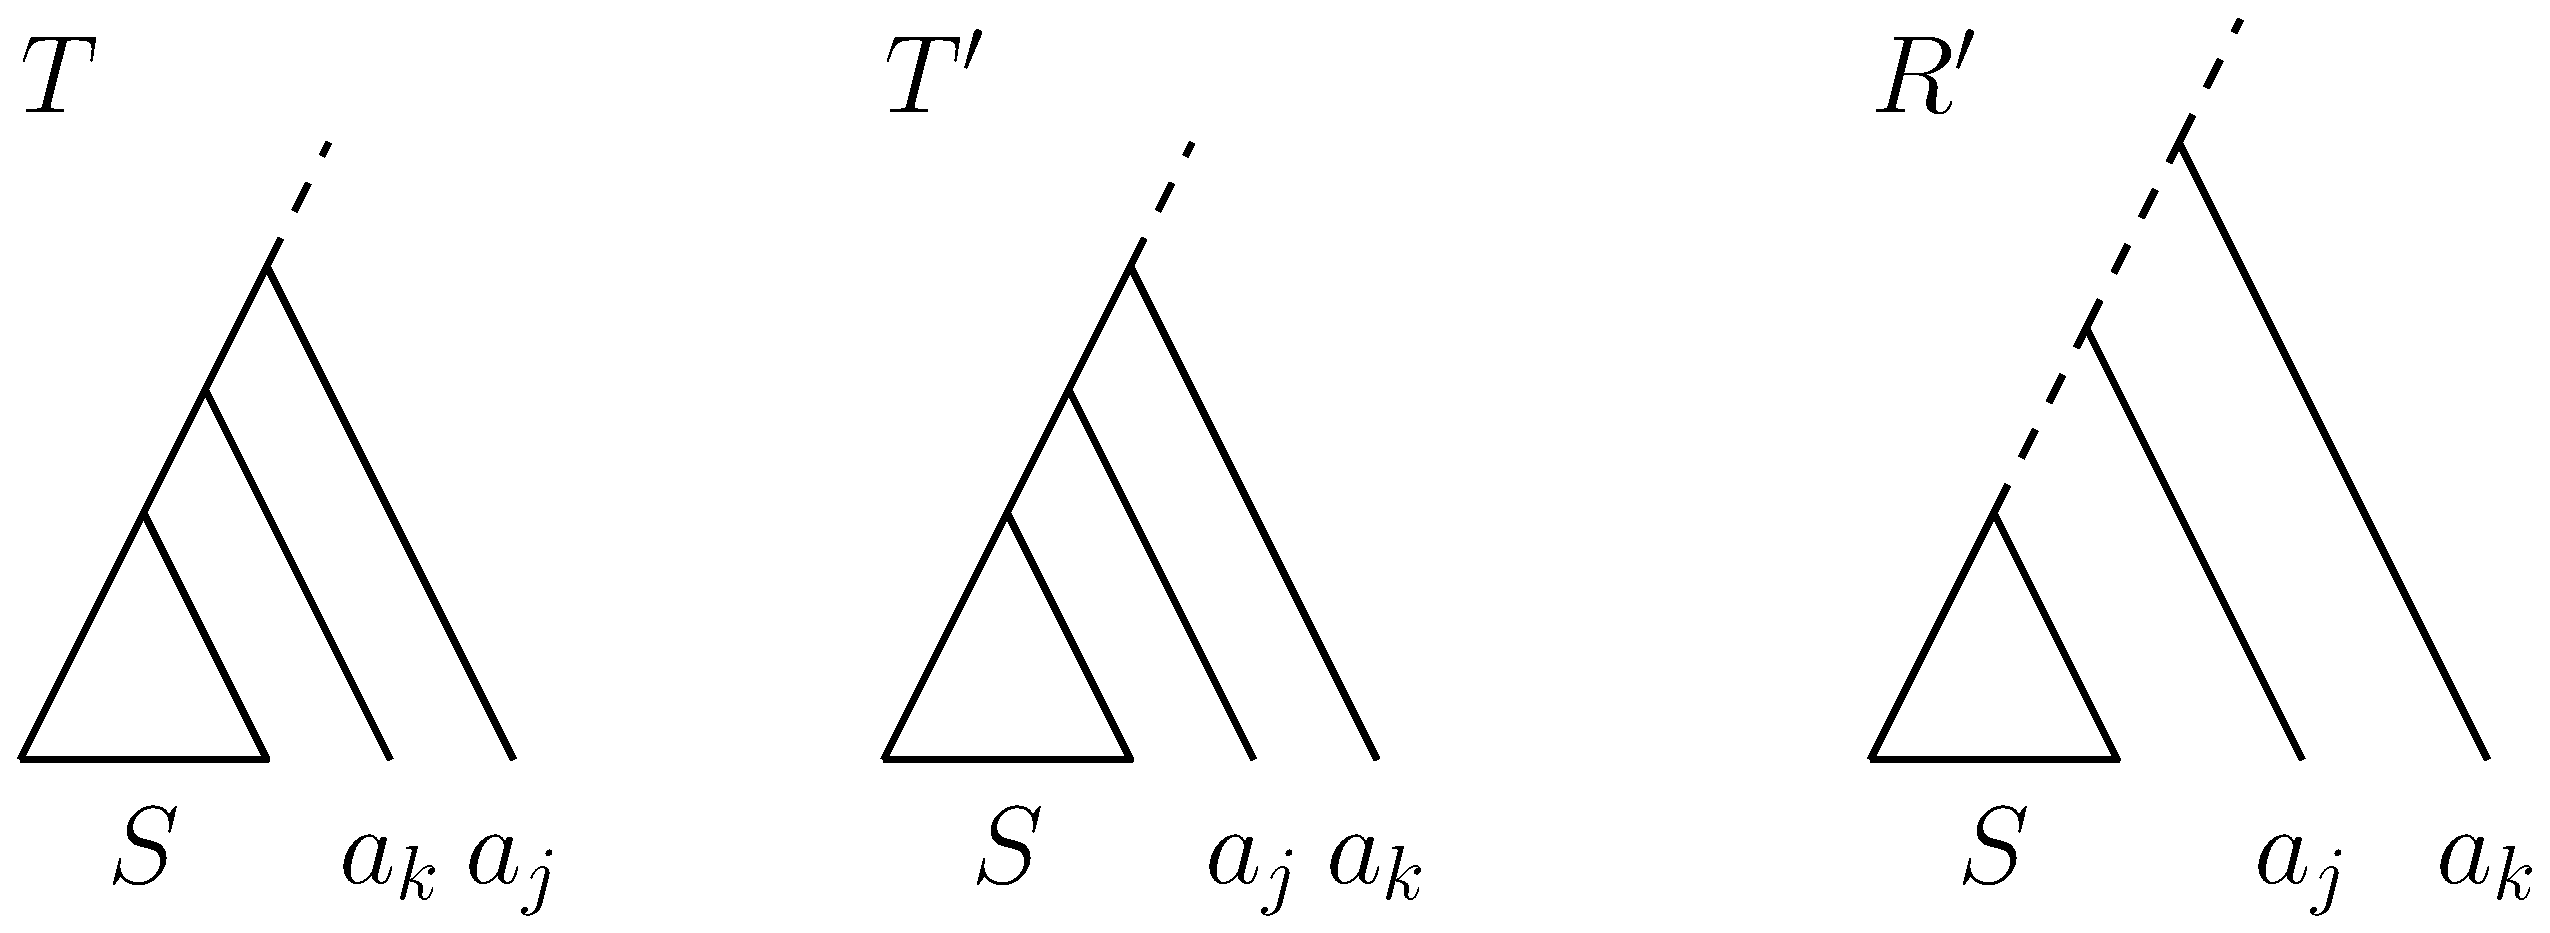
\includegraphics[width=0.66\textwidth]{proof_caterpillar_convex_rnni.eps}
		\caption{Trees $T$, $T'$, and $R'$ as described in the proof of \autoref{thm:caterpillar_convex_rnni}.
		All three trees share the subtree induced by subset $S$ of leaves.
		Between $T$ and $T'$ only leaves $a_j$ and $a_k$ are exchanged.
		Dashed lines represent remaining part of trees, which are equal in $T$ and $T'$.}
		\label{fig:proof_caterpillar_convex_rnni}
	\end{figure}

	We now compare the lengths of $\fp(R',T)$ and $\fp(R',T')$.
	By our assumptions on $T$, the clusters considered on $\fp(R,T)$ in the two iterations following $R'$ are $S \cup \{a_k\}$ and $S \cup \{a_k, a_j\}$.
	Decreasing the rank of $(S \cup \{a_k\})_{R'}$ takes $\rank(S \cup \{a_k\})_{R'} - (\rank(S)_{R'} + 1)$ $\rnni$ moves, the following iteration for $S \cup \{a_k, a_j\}$ takes $\rank(S \cup \{a_j\})_{R'} + 1 - (\rank(S)_{R'} + 2)$.
	In particular, the rank of the most recent common ancestor of $S \cup \{a_k, a_j\}$ equals the rank of the most recent common ancestor of $S \cup \{a_j\}$ after the first iteration following $R'$, as $a_j$ has parent with rank higher than $a_k$ at that point.
	Since the parents of $a_k$ and $a_j$ exchange while the rank of $(S \cup \{a_k\})_{R'}$ decreases, the rank of $(S \cup \{a_j\}$ decreases by one during that iteration, compared to $R'$.
	On $\fp(R,T')$ first $\rank(S \cup \{a_j\})_{R'} - (\rank(S)_{R'} + 1)$ $\rnni$ moves decrease the rank of $(S \cup \{a_j\})_{R'}$, and then $\rank(S \cup \{a_j, a_k\})_{R'} - (\rank(S)_{R'} + 2)$ are needed for $S \cup \{a_k, a_j\}$.

	Let $Q$ and $Q'$ be the trees on $\fp(R,T)$ and $\fp(R,T')$, respectively, after the two iterations following $R'$.
	By the above the number of moves on $\fp(R,T)$ between $R'$ and $Q$ is one higher than the number of moves on $\fp(R,T')$ between $R'$ and $Q'$.
	Since the trees $Q'$ and $T'$ can be received from permuting the leaves of $Q$ and $T$ by the same permutation, namely the transposition $(a_j, a_k)$, the distances between these pairs of trees coincide: $d(Q,T) = d(Q',T')$.
	We can conclude $d(R,T) = d(R,T') + 1$, and hence $T'$ is on a shortest path from $T$ to $R$.
\end{proof}

\todo{Why?}
The convexity of the set of caterpillar trees in $\dtt_m$ follows from \autoref{thm:caterpillar_convex_rnni}.

\begin{corollary}
	The set of caterpillar trees is convex in $\dtt_m$.
	\label{cor:caterpillar_convex_dtt}
\end{corollary}

\summary{With Theorem~\ref{thm:caterpillar_convex_rnni} we can find a more efficient way to compute distances between caterpillar trees.}
Using the convexity of the set of caterpillar trees (\autoref{thm:caterpillar_convex_rnni}), there are several algorithms of computing the distance between two caterpillar trees.

\todo{Do I need to go more into detail about TSP?}
A problem analogous to the shortest path problem for caterpillar trees is the \emph{Token Swapping Problem} (TSP) \autocite{Kawahara2017-ey} on a special class of graphs, so-called lollipop graphs.
The only moves possible between caterpillar trees are $\nni$ moves, which simply swap two leaves, and these can be translated to swapping two tokens in TSP.
\textcite{Kawahara2017-ey} provide an algorithm for TSP on lollipop graphs, which can be used for computing distances between caterpillar trees in $\rnni$ as well.
This algorithm however has worst-case time complexity $\O(n^2)$, the same as $\findpath$.

We are however able to present an algorithm with better worst-case complexity, specifically in $\O(n \log n)$ for $\rnni$ (\autoref{cor:caterpillar_distance_rnni_nlogn})
At first we present in \autoref{thm:caterpillar_distance_formula} a formula to express distances between two caterpillar trees in $\rnni$.
Using this, distances between caterpillar trees in $\dtt_m$ can be computed in $\O(m + n \log n)$ in $\dtt_m$ (\autoref{cor:caterpillar_distance_dtt_m_nlogn}).

\begin{theorem}
	Let $T$ and $R$ be caterpillar trees in $\rnni$ such that \[1 = \rank(a_1)_R = \rank(a_2)_R < \rank(a_3)_R < \ldots < \rank(a_n)_R = n-1\]
	and
	\[P_T := \{(i,j)| \rank(a_i)_T < \rank(a_j)_T \text{ and } \rank(a_i)_R > \rank(a_j)_R\},\]
	\begin{align*}
		M_T := &\{a_i| (\forall l \textnormal{ with } \rank(a_l)_T \leq \rank(a_i)_T: \rank(a_l)_R > \rank(a_i)_r)\} \\
		& \cap \{a_i | \rank(a_i)_T < \min\{\rank(a_1)_T, \rank(a_2)_T\}\}
	\end{align*}
	Then it is
	\[d(T,R) = p_T - m_T,\]
	for ${m_T = |M_T|}$ and ${p_T = |P_T|}$.
	\label{thm:caterpillar_distance_formula}
\end{theorem}

We refer to pairs $(i,j) \in P_T$, as defined in \autoref{thm:caterpillar_distance_formula}, as transpositions.
The reason for this is that the caterpillar trees can be seen as permutations of the set $\{a_1, \ldots, a_n\}$, ordered according to increasing rank of their parents.
The tree $R$ then corresponds to the identity permutation $(a_1, a_2, a_3, \ldots, a_n)$.
We therefore call elements in $P_T$ transpositions.
Note that there is no one-to-one correspondence between permutations and caterpillar trees.
For example the permutation $(a_2, a_1, a_3, \ldots, a_n)$ corresponds to the tree $R$ as well, as the first two elements share a parent in the caterpillar tree.
Therefore, the two pairs that share parents in $T$ and $R$, respectively, are not in the set $P_T$.

\begin{proof}
	Let $T$ and $R$ be caterpillar trees as described above and $\hat d(T,R) = p_T - m_T$.
	For proving $\hat d(T,R) = d(T,R)$, it is sufficient to show that for all caterpillar trees $T'$ that are neighbour of $T$ it is
	\begin{align}
		\hat d(T',R) \geq \hat d(T,R) - 1.
		\label{eq:distance_proof}
	\end{align}
	That $\hat d$ and $d$ coincide follows by induction.

	For proving Inequality~\ref{eq:distance_proof} we first establish $p_{T'} \geq p_T - 1$ and then $m_{T'} \leq m_t + 1$, assuming that $T'$ is a caterpillar tree that is $\rnni$ neighbour of $T$.
	We then show that it cannot be $p_{T'} = p_T - 1$ and $m_{T'} = m_t + 1$, which proves Inequality~\ref{eq:distance_proof}.
	Throughout this proof we call pairs $(i,j) \in P_T$ transpositions, as the order of ranks of parents of leaves in the caterpillar trees $T$ and $T'$ can be seen as a permutation of their order in $R$.

	It is $p_{T'} \geq p_T - 1$, because the only move possible between caterpillar trees $T$ and $T'$ is an $\nni$ move exchanging two leaves, and hence at most one transposition of $T$ can be resolved in $T'$.
	Let $a_k, a_j$ be the leaves that exchange their position between $T$ and $T'$, such that $\rank(a_k)_T < \rank(a_j)_T$.
	Since these are the only leaves that change positions between $T$ and $T'$, they are the only elements that could be in $M_{T'} \setminus M_T$.
	It remains to show $(M_{T'} \setminus M_T) \neq \{a_k, a_j\}$, from which we can follow that $m_{T'} \leq m_T - 1$.
	We prove this by showing that if $a_k \in (M_{T'} \setminus M_T)$, it follows $a_j \notin M_{T'}$.

	We assume that $a_k \in (M_{T'} \setminus M_T)$, implying $a_k \notin M_T$, so at least one of the following conditions must be violated for $i = k$:
	\setcounter{equation}{0} % Set counter for equation to get C1 and C2 for conditions
	\renewcommand{\theequation}{C\arabic{equation}}
	\begin{align}
		\forall l \text{ with } \rank(a_l)_T \leq \rank(a_i)_T: \rank(a_l)_R > \rank(a_i)_R \label{condition1}\\
		\rank(a_i)_T < \min\{\rank(a_1)_T, \rank(a_2)_T\}.
		\label{condition2}
	\end{align}
	% reset counter for future uses
	\setcounter{equation}{1}
	\renewcommand{\theequation}{\arabic{equation}}

	At first we consider the case that (\ref{condition1}) is violated for $a_k$ in $T$.
	Then there is an $l$ such that $\rank(a_l)_T \leq rank(a_k)_T$ and $\rank(a_k)_R > \rank(a_l)_R$.
	It immediately follows that the same condition is violated for $a_k$ in $T'$, because the $\nni$ move exchanging $a_k$ and $a_j$ preserves the relationship of $a_k$ and $a_l$, as $l \neq j$.
	It hence is $a_k \notin M_{T'}$, contradicting our assumption $a_k \in (M_{T'} \setminus M_T)$.

	We can therefore assume that (\ref{condition2}) is violated for $a_k$ to not be in $M_T$.
	It follows $\rank(a_k)_T \geq \min\{\rank(a_1)_T, \rank(a_2)_T\}$.
	As only $a_k$ and $a_j$ exchange between $T$ and $T'$ and $a_k \in M_{T'}$, it follows $a_j \in \{a_1, a_2\}$.
	This however results in a violation of (\ref{condition2}) for $a_j$ in $T'$ and hence $a_j \notin M_{T'}$.
	We can conclude $(M_{T'} \setminus M_T) \neq \{a_k, a_j\}$, and hence $m_{T'} \leq m_T + 1$.

	It remains to show that it cannot be $p_{T'} = p_T - 1$ and $m_{T'} = m_T + 1$ at the same time, in order to prove Inequality~\ref{eq:distance_proof}.
	We assume $p_{T'} = p_T - 1$, hence $(k,j)$ is a transposition in $T$, meaning that $\rank(a_k)_T < \rank(a_j)_T$ and $\rank(a_k)_R > \rank(a_j)_R$.
	As $a_k$ and $a_j$ are the only leaves that could be in $M_T \setminus M_{T'}$, it suffices to show that none of them actually are in $M_{T'} \setminus M_T$, resulting in $m_{T'} < m_T + 1$.

	That $a_k$ is not in $M_{T'}$ follows from a violation of (\ref{condition2}) by $\rank(a_j)_{T'} < \rank(a_k)_{T'}$ and $\rank(a_j)_R < \rank(a_k)_R$, and hence it is $a_k \notin M_{T'} \setminus M_T$.
	Moreover, if $a_j \in M_{T'}$, it follows $a_j \in M_{T'}$ as explained in the following, which yields $a_j \notin M_{T'} \setminus M_T$.
	If $a_j \in M_{T'}$, both conditions (\ref{condition1}) and (\ref{condition2}) are met by $a_j$ in $T'$.
	With $\rank(a_k)_T < \rank(a_j)_T$ and $\rank(a_k)_R > \rank(a_j)_R$ it immediately follows that these conditions are also met in $T$, and hence $a_k \in M_T$, and therefore $a_k \notin M_{T'} \setminus M_T$.

	Concluding, it is $M_{T'} \setminus M_T = \emptyset$, and we can follow that if $p_{T'} = p_T - 1$, it is $m_{T'} < m_T + 1$, which concludes this proof.
\end{proof}

\todo{Can this somehow be used in $\dtt_m$?}

\begin{corollary}
	The distance between two caterpillar trees can be computed in $\O(n \log n)$ in $\rnni$.
	\label{cor:caterpillar_distance_rnni_nlogn}
\end{corollary}

\begin{proof}
	By \autoref{thm:caterpillar_distance_formula} the distance between two caterpillar trees is the number of transpositions between two sequences of length $n$ minus the variable $m_T$ as defined in \autoref{thm:caterpillar_distance_formula}.
	The value $m_T$ can be computed time linear in $n$ for any caterpillar tree $T$ by considering the leaves of the tree ordered according to increasing rank of their parents.
	The number of transpositions of a sequence of length $n$ (Kendall-tau distance) can be computed in time $\O(n \log n)$ \autocite{Knight1966-hx}.
	This number is equivalent to $p_t$, as defined in \autoref{thm:caterpillar_distance_formula}, when ignoring the potential transpositions for the pairs of leaves sharing a parent in $T$ and $R$, respectively.
	The worst-case running time for computing the $\rnni$ distance between caterpillar trees is therefore $\O(n \log n)$.
\end{proof}

\subsection{Diameter and Radius}

\summary{Definition of Diameter.}
In this section we  investigate the \emph{diameter} of $\rnni$ and $\dtt_m$, which is the greatest distance between any pair of vertices (trees) in each of these graphs, respectively, i.e. $\max\limits_{\text{trees }T,R}d(T,R)$.
We first establish the exact diameter of $\rnni$, improving the upper bound $n^2 - 3n - \frac{5}{8}$ given by \textcite{Gavryushkin2018-ol}.
Afterwards, we generalise this result to $\dtt_m$.

\begin{theorem}
	The diameter of $\rnni$ is $\frac{(n-1)(n-2)}{2}$.
	\label{thm:diameter_rnni}
\end{theorem}

\begin{proof}
	For proving this theorem we use the fact that $\findpath$ computes shortest paths in $\rnni$.
	Each iteration $i$ of $\findpath$, applied to two trees $T$ and $R$ in $\rnni$, decreases the rank of the most recent common ancestor of a cluster $C$ of $R$ in the currently last tree $T'$ on the already computed path (starting wth $T' = T$).
	The maximum rank of $(C)_{T'}$ at the beginning of iteration $i$ is $n-1$, the rank of the root.
	As every move decreases the rank of $(C)_{T'}$ by one, there are at most $m-i$ moves needed in iteration $i$.
	The maximum length of a shortest path in $\rnni$ is hence $\sum \limits_{i = 1}^{n-1} i = \frac{(n-1)(n-2)}{2}$.
	Note that the caterpillar trees $[\{a_1, a_2\}, \{a_1, a_2, a_3\}, \ldots, \{a_1, \ldots, a_n\}]$ and $[\{a_n, a_{n-1}\}, \{a_n, a_{n-1}, a_{n-2}\}, \ldots, \{a_n, \ldots, a_1\}]$ provide an example of trees that have distance $\frac{(n-1)(n-2)}{2}$, as already pointed out in \autocite[Corollary 1]{Collienne2020-iu}, proving that this upper bound for the length of a shortest path is tight.
\end{proof}

\todo{The order of this and the previous theorem needs to change again, we can't rely on the formula for $l(T,R)$.
Instead, use $\findpath$ and what we know about the extended ranked versions of the trees}
% Use the decomposition of $\fp(T,R)$ into $\rnni$ and length moves
% The maximum number of these moves is the diameter of $\rnni$, which is $\frac{(n-1)(n-2)}{2}$.
% Then count the number of possible length moves, which are rank moves with $T_c$.
% The maximum here is reached when every node from subtree $T$ swaps rank with every node of subtree $T_c$.
% This number is $(n-1)(m-n-1)$.
% Sum of both is $m(n-1) - \frac{n(n-1)}{2}$, proof finished.
\begin{theorem}
	The diameter of $\dtt_m$ is $m(n-1) - \frac{n(n-1)}{2}$.
	\label{thm:dtt_diameter}
\end{theorem}

\begin{proof}
	With \autoref{lemma:dtt_fp_path_rnni} we know that the distance between two trees $T$ and $R$ in $\dtt_m$ is the sum of the minimum number $r(T,R)$ of $\rnni$ moves and the minimum number $l(T,R)$ of length moves on any shortest path between them.
	We furthermore have seen (\autoref{thm:diameter_rnni}), that the diameter of $\rnni$ is $\frac{(n-1)(n-2)}{2}$, which is the maximum number that $r(T,R)$ can be for trees $T$ and $R$ in $\dtt_m$.
	We now establish the maximum of $l(T,R)$ for two trees $T$ and $R$ and will see afterwards, that there are actually trees which reach maxima for both $r(T,R)$ and $l(T,R)$.

	We have already seen in the proof of \autoref{lemma:dtt_fp_path_rnni} that it is $l(T,R) = \sum_{i = n+1}^{m+2} |\rank(a_{i})_{T_c} - \rank(a_{i})_{R_c}|$, where $T_c$ and $R_c$ are the caterpillar trees added to $T$ and $R$ when applying \autoref{alg:ranked_tree}, respectively.
	The maximum number of length moves is reached when on $\findpath$ between $T_r$ and $R_r$ all internal nodes of the newly added caterpillar tree swap rank with all internal nodes of the subtree on the original leaf set $\{a_1, \ldots, a_n\}$.
	Since these two subtrees have $m-n+1$ and $n-1$ internal nodes, respectively, the maximum number for $l(T,R)$ between any two trees in $\dtt_m$ is $(n-1)(m-n+1)$.

	The sum of the maximum number for $r(T,R)$ and $l(T,R)$ is hence $\frac{(n-1)(n-2)}{2} + (n-1)(m-n+1) = m(n-1) - \frac{n(n-1)}{2}$.
	That this upper bound is actually the diameter of $\dtt_m$ can be proven by the trees in \autoref{fig:cat_max_dist_dtt} for which the path computed by $\findpath$ has length $m(n-1) - \frac{n(n-1)}{2}$.
	\begin{figure}[ht]
		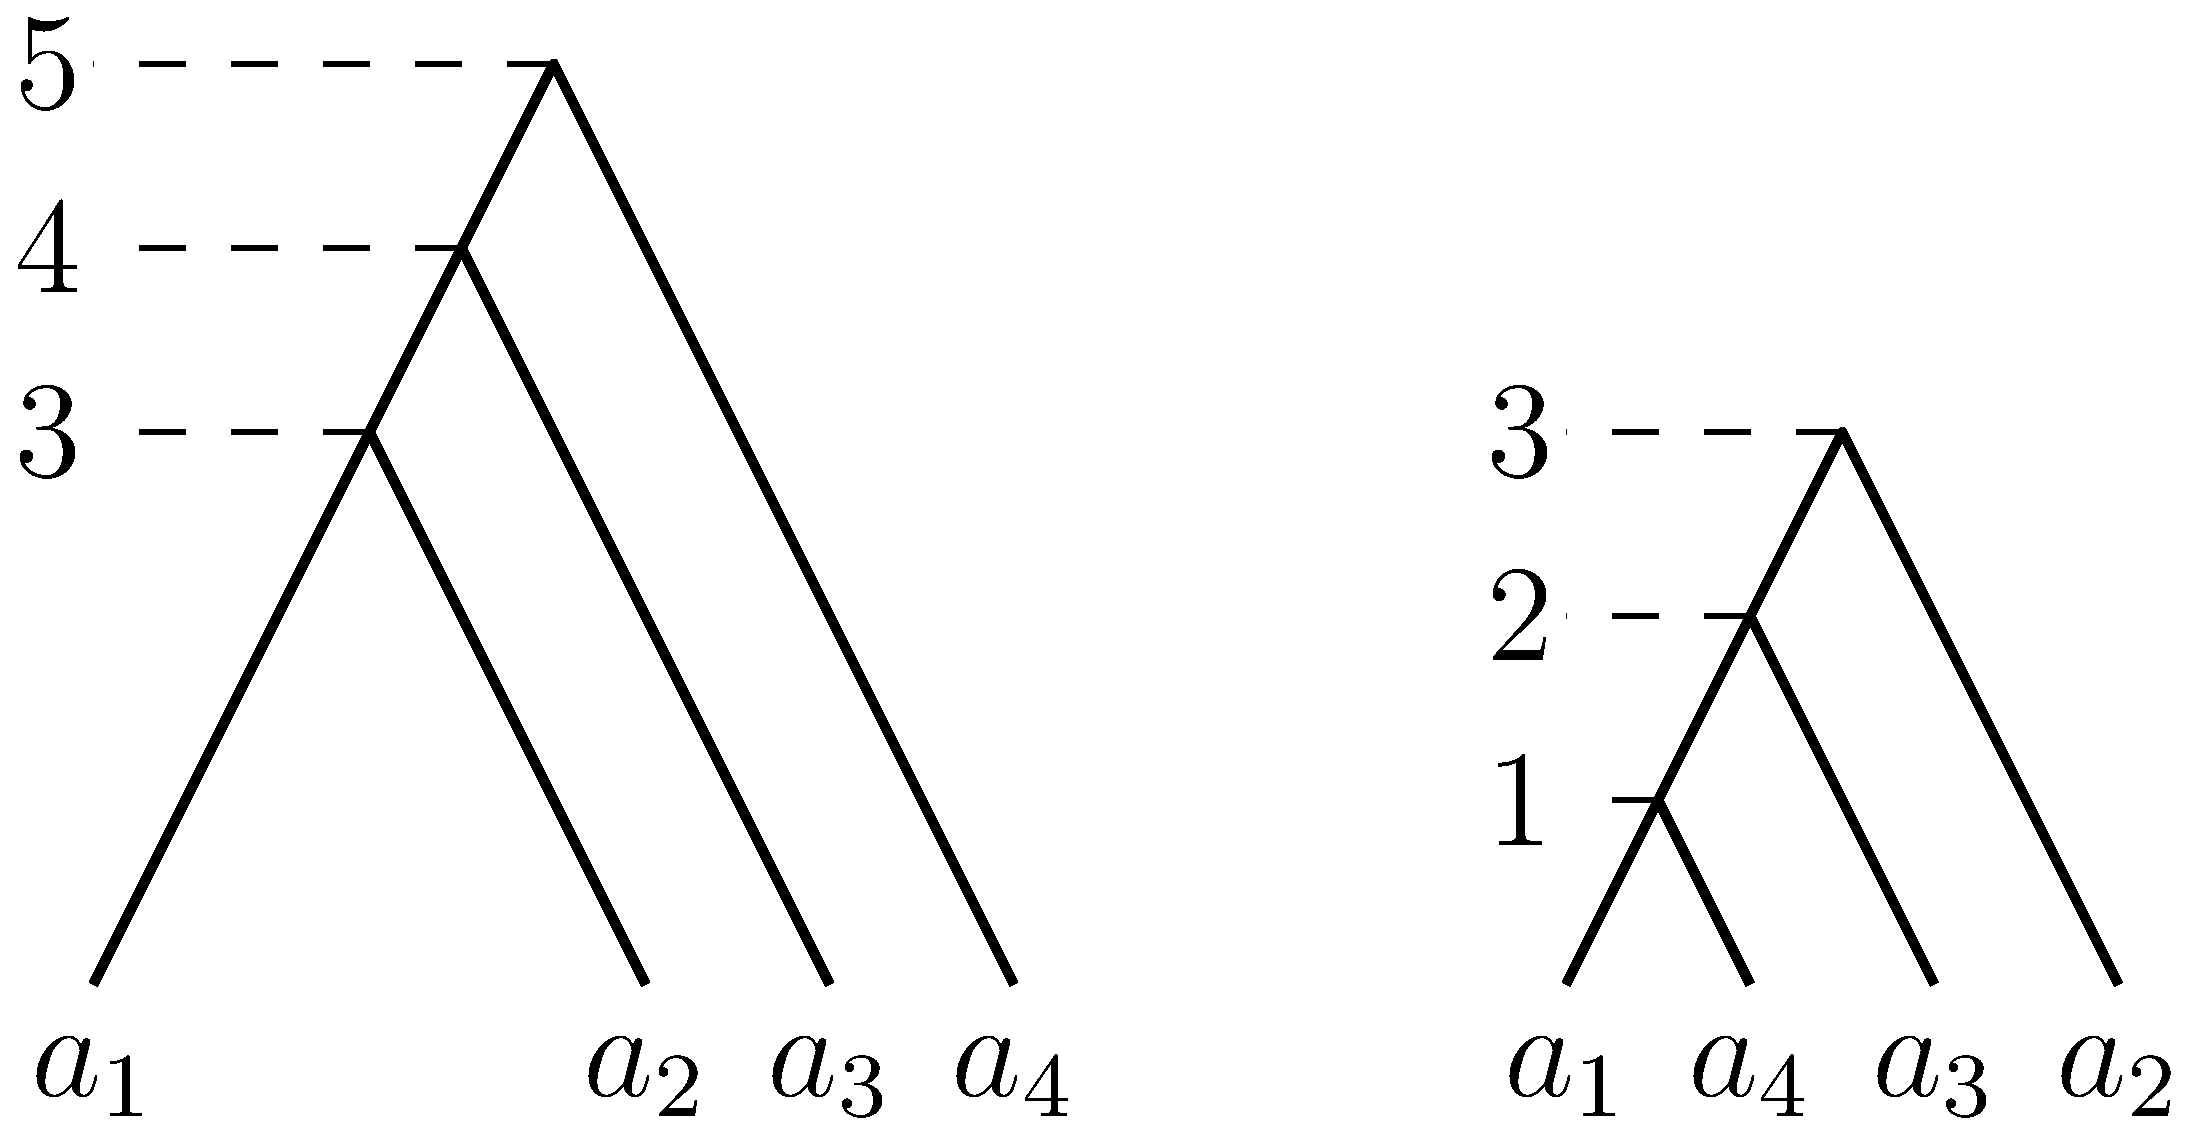
\includegraphics[width=0.65\textwidth]{cat_max_dist_dtt.eps}
		\caption{Trees with distance $m(n-1) - \frac{n(n-1)}{2}$}
		\label{fig:cat_max_dist_dtt}
	\end{figure}
\end{proof}

Since the $\rnni$ graph is the graph $\dtt_{n-1}$, the diameter of $\rnni$ is a direct result of \autoref{thm:dtt_diameter}.
Note that the worst-case running time of $\findpath$ is $\O(n^2)$ and $\O(nm)$ in $\rnni$ and $\dtt_m$, respectively, and only depends on the diameter of the corresponding tree spaces.
For computing a shortest path, there is no algorithm with better worst-case running time than this, as the running time for algorithms computing shortest paths is bounded from below by the diameter of the corresponding space.

\summary{Radius of $\rnni$ is equal to its diameter.}
The \emph{radius} of a graph is defined as he minimum distance of any vertex in the graph to the vertex with maximum distance from it.
For $\dtt_m$ and $\rnni$, this is $\min\limits_{\text{tree } T}\max\limits_{\text{tree }R} d(T,R)$, where $d$ is a distance measure in the corresponding graph.
In the following we see that the radius of $\rnni$ equals its diameter, which we show to not be true for $\dtt_m$ afterwards.

\begin{lemma}
	The radius of $\rnni$ equals its diameter, that is $\frac{(n-1)(n-2)}{2}$.
	\label{lemma:radius_rnni}
\end{lemma}

\begin{proof}
	We prove this lemma by showing that every tree $T$ in $\rnni$ has a caterpillar tree $R$ with distance $\frac{(n-1)(n-2)}{2}$ to $T$.
	This will be proven by induction on the number of leaves $n$.

	The base case $n=3$ is trivial, as all three trees in this space are caterpillar trees with distance one from every other tree.
	For the induction step we consider an arbitrary tree $T$ with $n+1$ leaves.
	Let $x$ and $y$ be the leaves of $T$ that share the internal node of rank one as parent in $T$, and let $T'$ be the tree on $n$ leaves resulting from deleting one of these leaves, say $x$, of $T$.
	By the induction hypothesis there is a caterpillar tree $R'$ with distance $\frac{(n-1)(n-2)}{2}$ to $T'$.
	Now consider the tree $R$ resulting from adding $x$ at the top of $R'$ such that the root of $R$ has $x$ and $R'$ as children.

	We noe consider the path computed by $\findpath$ from $T$ to $R$.
	In the first iteration of $\findpath$, $(\{x,y\})_R$ moves down until it reaches rank one.
	Therefore, first $(x)_R$ moves down by $\nni$ moves until it reaches rank one more than $(y)_R$.
	Then a further $\nni$ move creates an internal node with children $x$ and $y$, before this node is moved down by rank swaps as depicted in Figure~\ref{fig:max_dist_ctree}.
	Altogether, there are $n-1$ $\rnni$ moves needed in the first iteration, as the rank of the parent of $x$ decreases by one within every move, starting at the root with rank $n$ and ending at the internal node of rank one.
	The tree at the end of this first iteration on $\fp(T,R)$ is identical to $R'$ when removing the leaf $x$ and suppressing its parent (the root, making the remaining child the new root).
	Since the cluster $\{x,y\}$ is not considered again in $\findpath$, the remaining part of $\fp(T,R)$ contains the same moves as $\fp(T',R')$, and hence $|\fp(T,R)| = |\fp(T',R')| + n-1$.
	Therefore it is $d(T,R) = \frac{(n-1)(n-2)}{2} + n-1 = \frac{n(n-1)}{2}$, which proves the lemma.
	\begin{figure}[ht]
		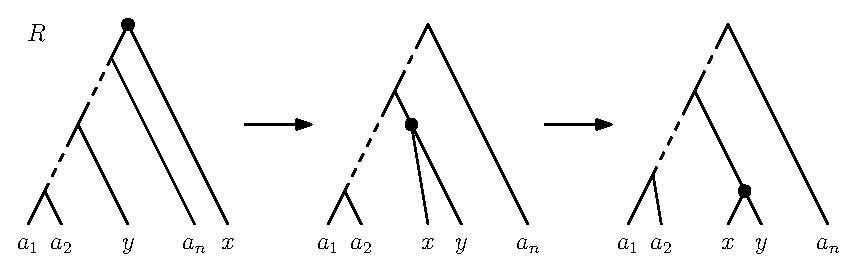
\includegraphics[width=0.8\textwidth]{max_dist_ctree.eps}
		\caption{Initial $n - 1$ $\rnni$ moves of $\fp(R,T)$ as described in the proof of Lemma~\ref{lemma:radius_rnni}.
		Removing the leaf $x$ and suppressing the non-root node of degree two from the tree on the right results in $R'$ as described in the lemma.}
		\label{fig:max_dist_ctree}
	\end{figure}
\end{proof}

Unlike in $\rnni$, the radius of $\dtt_m$ does not equal its diameter.
A counterexample is given by the tree depicted in \autoref{fig:dtt_radius_counterexample} on three leaves in $\dtt_4$.
There is no tree in $\dtt_4$ that has distance $m(n-1) - \frac{n(n-1)}{2}$ (diameter of $\dtt_m$) from that tree.

\begin{figure}[ht]
	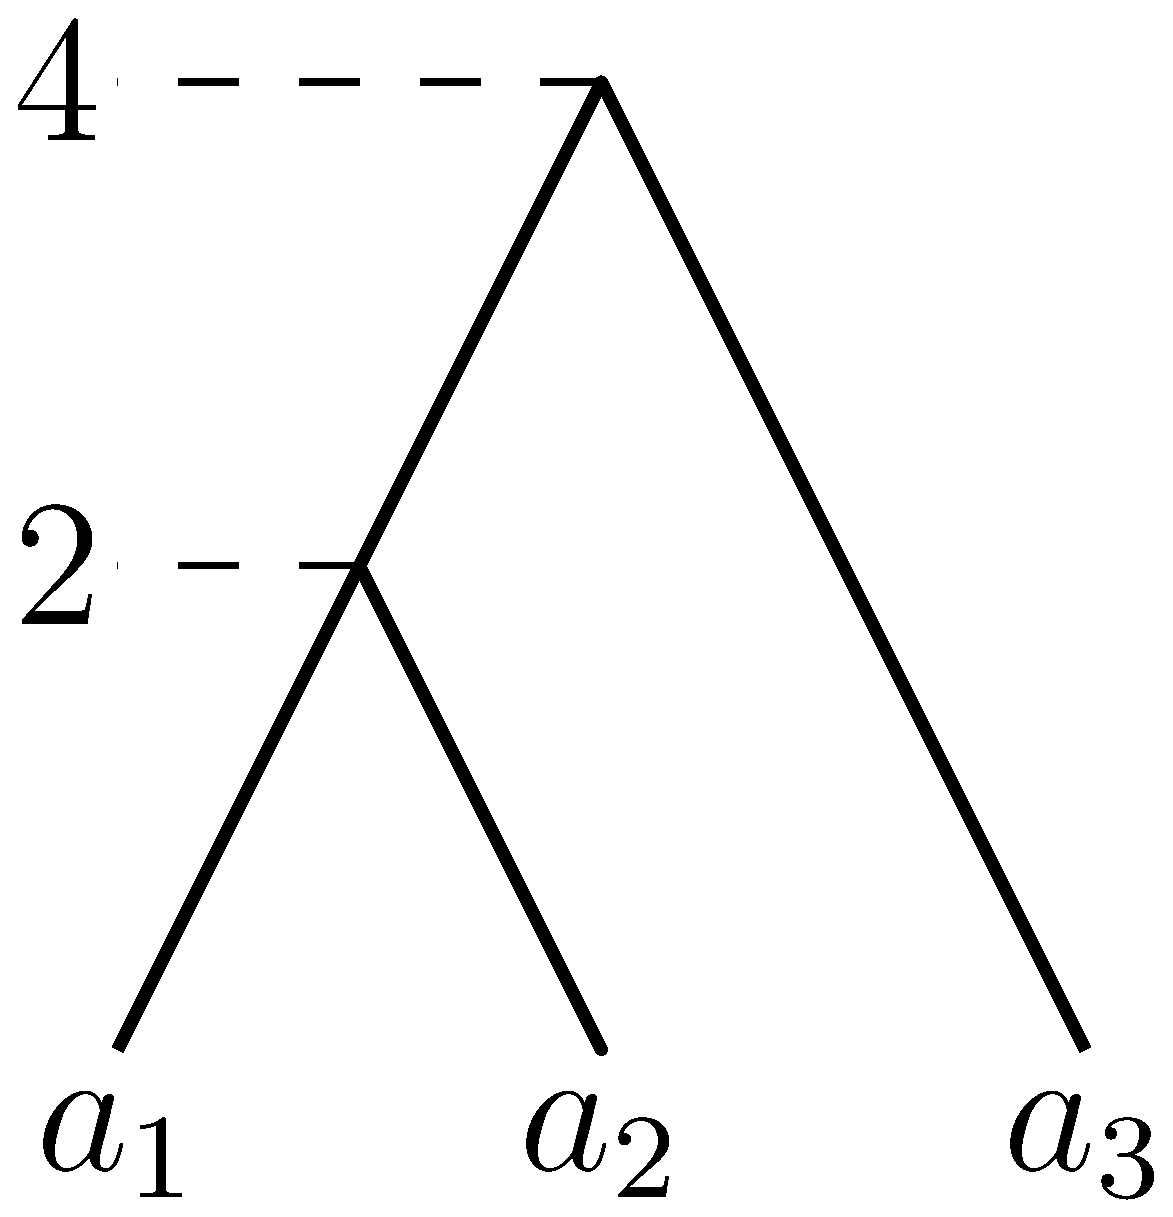
\includegraphics[width=0.15\textwidth]{dtt_radius_counterexample.eps}
	\caption{Tree in $\dtt_4$ on three leaves for which there is not tree with distance $5 = m(n-1) - \frac{n(n-1)}{2}$ (diameter) from it}
	\label{fig:dtt_radius_counterexample}
\end{figure}


\section{Discussion}

\summary{How partition lattices correspond to $\rnni$.}

\summary{Implementation of FP}

\subsection{Open Problems}

\summary{More efficient algorithm for computing distances (not shortest paths) -- mentioning David's results on mapping onto L1?}

\summary{Radius $\dtt_m$}

\summary{$\rnni(rho)$ and parameter $\rho$ for discrete time-trees}

\summary{scaling-free tree space}

\end{document}